\documentclass{IOS-Book-Article}
\usepackage{amssymb}
\usepackage{array}
\usepackage{graphics}
\usepackage{graphicx}
\usepackage{indentfirst}
\usepackage{enumerate}
\usepackage{listings}
\usepackage{color}
\usepackage{tabularx}
\usepackage{supertabular}
\usepackage{longtable}
\usepackage{natbib}
\usepackage{enumerate}
\usepackage{changepage}
\usepackage{enumitem}
\setenumerate[1]{itemsep=0pt,partopsep=0pt,parsep=\parskip,topsep=0pt}
\setitemize[1]{itemsep=0pt,partopsep=0pt,parsep=\parskip,topsep=0pt}

\DeclareFixedFont{\mf}{T1}{cmbr}{m}{n}{10pt}

\lstset{ %
  language=Octave,                 % the language of the code
  basicstyle=\footnotesize,            % the size of the fonts that are used for the code
 % numbers=left,                    % where to put the line-numbers
 % numberstyle=\tiny\color{gray},   % the style that is used for the line-numbers
  stepnumber=2,                    % the step between two line-numbers. If it's 1,  each line 
                                  % will be numbered
  numbersep=5pt,                   % how far the line-numbers are from the code
  backgroundcolor=\color{white},       % choose the background color. You must add \usepackage{color}
  showspaces=false,                % show spaces adding particular underscores
  showstringspaces=false,          % underline spaces within strings
  showtabs=false,                  % show tabs within strings adding particular underscores
  frame=single,                    % adds a frame around the code
  rulecolor=\color{black},         % if not set,  the frame-color may be changed on line-breaks within not-black text (e.g. commens (green here))
  tabsize=2,                       % sets default tabsize to 2 spaces
  captionpos=b,                    % sets the caption-position to bottom
  breaklines=true,                 % sets automatic line breaking
  breakatwhitespace=false,         % sets if automatic breaks should only happen at whitespace
  title=\lstname,                    % show the filename of files included with \lstinputlisting;
                                  % also try caption instead of title
%  keywordstyle=\color{blue},           % keyword style
%  commentstyle=\color{dkgreen},        % comment style
 % stringstyle=\color{mauve},          % string literal style
  escapeinside={\%*}{*)},             % if you want to add LaTeX within your code
  morekeywords={*, ...}               % if you want to add more keywords to the set
}





\begin{document}

\pagestyle{headings}
\def\thepage{}

\begin{frontmatter} 

\title{Checking the validity of rule-based arguments grounded in cases: \\a computational approach}

%\markboth{}{September 2018\hb}
%\subtitle{Subtitle}

\author[A]{\fnms{Heng} \snm{Zheng}}, \author[B]{\fnms{Minghui} \snm{Xiong}} and \author[A]{\fnms{Bart} \snm{Verheij}\thanks{Corresponding Author: Artificial Intelligence, University of Groningen, The Netherlands; E-mail:bart.verheij@rug.nl.}}

\runningauthor{H. Zheng et al.}
\address[A]{Artificial Intelligence, University of Groningen, The Netherlands}
\address[B]{Institute of Logic and Cognition, Sun Yat-sen University, Guangzhou, China}

\begin{abstract}
Legal justice needs judges' decisions to be rational and reasonable in the sense that arguments are based on rules and grounded in cases.  One puzzle studied in AI \& Law is how arguments, rules and cases are formally connected. Recently a formal theory was proposed formalizing how the validity of arguments based on rules can be grounded in cases. Three kinds of argument validity were distinguished: coherence, presumptiveness and conclusiveness. In this paper the theory is implemented in a Prolog program. We test the theory using two case studies: the first is a model of Dutch tort law developed earlier; the second is a newly developed model of Chinese copyright infringement law. The case studies illustrate that by the use of the implementation the process of modeling becomes more efficient and less error-prone.
\end{abstract}

\begin{keyword}
Artificial Intelligence and Law\sep Rule-based Reasoning\sep Case-based Reasoning\sep Argumentation Modeling\sep Prolog
\end{keyword}
\end{frontmatter}
%\markboth{September 2018\hb}{September 2018\hb}

\section{Introduction}
\noindent 
%Legal justice requires judges to give reasonable decisions. AI technologies can support the reduction of the number of  cases in which people were unjustly charged by verifying the rationality and validity of judges' decisions automatically. 
In the field of AI and law---going at least back to the 1970s \cite{Buchanan1970Some}---, scholars usually follow three approaches to develop legal reasoning systems, which are rule-based reasoning, case-based reasoning and argument-based reasoning. 
%The study of legal reasoning systems . Scholars developed various systems by following rule-based reasoning, case-based reasoning and argument-based reasoning. 
In the 1980s, the British Nationality Act (BNA) was implemented in Prolog~\citep{Sergot1986The}, in a successful attempt to develop rule-based reasoning systems in the field of law. Case-based reasoning was modeled in the systems HYPO, BankXX, CATO and IBP~\citep{risslandAshley1987,Ashley1991Reasoning,Rissland1996BankXX,Aleven1997Evaluating,Bruninghaus2003Predicting}. 
CABARET \citep{Rissland1991CABARET} and GREBE \citep{Branting1991Building} are hybrid systems not only use case-based reasoning, but also other kinds of reasoning. 
%\citep{Bench-Capon2017HYPO}.
Argumentation models of legal rule-based and case-based reasoning~\citep{prakkenSartor1996,prakkenSartor1998} are connected to later systems based on abstract argumentation~\citep{Dung1995On}, inspiring for instance ASPIC+ \citep{Prakken2010An}, ABA \citep{Bondarenko1997An} and DeLP \citep{Garcia2003Defeasible}.

The recent case model formalism \citep{Verheij2016Correct} is a hybrid theory showing connections between cases, rules and arguments~\citep{Verheij2017Formalizing}. The formalism defines different ways in which rule-based arguments can be valid in cases: arguments can be coherent, conclusive or presumptive. The formalism has been applied to model Dutch tort law, showing how a rule-based legal domain can be grounded in legal cases. In this way, a formal connection is established between the civil law tradition focusing on rules and the common law tradition focusing on cases. The formalism has also been applied to the modeling of a series of New York tort cases (as studied by~\cite{bermanHafner1995,hafnerBerman2002}), analyzing value-guided teleological reasoning~\citep{Verheij2016Formalizing}.

%This formalism also incorporates ideas from value judgements, it could be used for comparing the arguments implicated in a case model and deciding which argument is more presumptive. However, the models in legal domain based on Verheij's theory often have complex argument structure. For users, it is easy to make mistakes through the original hand-made way during the process of modeling. Thus using a program to verify the model and the arguments implicated by it is necessary. 
%The theory background of this paper comes from Bart Verheij's research on case model formalism \citep{Verheij2016Correct}. In this formalism, three kinds of argument validity in the case model can be analyzed through a given preferred relation of the cases. 
%Verheij's theory has incorporated the notion of values in argumentation and also combines rules, cases and arguments together which can be applied in the field of law \citep{Verheij2017Formalizing} and used for ethical systems design \citep{Verheij2016Formalizing}.

The present paper provides a computational version of the case model formalism. A Prolog program is presented that can computationally check whether a case model is correct, whether rule-based arguments are valid (in the three kinds of validity coherence, conclusiveness and presumptiveness), and whether defeating circumstances are rebutting, undercutting or undermining. The computational tool can be used to support the manual modeling of a complex legal domain, making that more manageable. As an example, we provide a new domain model, namely Chinese copyright infringement law, both formally (as a case model) and computationally (in Prolog).

\section{Verheij's case model formalism}

\noindent Verheij's case model formalism was first introduced in \citep{Verheij2016Correct}. Verheij uses a classical formal logic  language $L$ generated from a set of propositional constants in a standard way. Verheij writes $\neg$ for negation, $\wedge$ for conjunction, $\vee$ for disjunction, $\leftrightarrow$ for equivalence, $\top$ for a tautology, and $\bot$ for a contradiction. The associated classical, deductive, monotonic consequence relation is denoted $\vDash$. Verheij assumes a finitely generated language. 

Verheij defines case models by the way of formalizing the idea of cases and their preferences. The cases in a case model must be logically consistent, mutually incompatible and different; and the comparison relation must be total and transitive. Here follows the definitions of case models addressed by Verheij.

\textbf{Definition 2.1}: A \textit{case model} is a pair $(C,  \geq)$ with finite $C \in L$, such that the following hold, for all $\varphi$, $\psi$ and $\chi \in C$: 
\begin{enumerate}
\item $\not \vDash \neg \varphi$;
\item If $\not \vDash \varphi \leftrightarrow \psi$, then $\vDash \neg$ ($\varphi \wedge \psi$);
\item If $\vDash \varphi \leftrightarrow \psi$, then $\varphi = \psi$;
\item $\varphi \geq \psi$ or $\psi \geq \varphi$;
\item If $\varphi \geq \psi$ and $\psi \geq \chi$, then $\varphi \geq \chi$.
\end{enumerate}

\textbf{Definition 2.2} (\textit{Arguments}) An \textit{argument} is a pair $(\varphi, \psi)$ with $\varphi$ and $\psi \in L$. The sentence $\varphi$ expresses the argument's premises, the sentence $\psi$ its conlusions, and the sentence $\varphi \wedge \psi$ the \textit{case made} by the arguments. Generalizing, a sentence $\chi \in L$ is a \textit{premise} of the argument when $\varphi \vDash \chi$, a \textit{conclusion} when $\psi \vDash \chi$, and a \textit{position} in the case made by the argument when $\varphi \wedge \psi \vDash \chi$. An argument $(\varphi, \psi)$ is \textit{(properly) presumptive} when $\varphi \not \vDash \psi$; otherwise \textit{not-presumptive}. An argument $(\varphi, \psi)$ is a \textit{presumption} when $\vDash \varphi$, i.e., when its premises are logically tautologous.

\textbf{Definition 2.3} \textit{(Coherent arguments)} Let $(C,  \geq)$ be a case model. Then we define, for all $\varphi$ and $\psi \in L$:

$(C,  \geq) \vDash (\varphi,  \psi)$ if and only if $\exists \omega \in C: \omega \in \varphi \wedge \psi$.

We then say that the argument from $\varphi$ to $\psi$ is \textit{coherent} with respect to the case model.

\textbf{Definition 2.4} (\textit{Conclusive arguments}) Let $(C,  \geq)$ be a case model. Then we define, for all $\varphi$ and $\psi \in L$:

$(C,  \geq) \vDash \varphi \Rightarrow \psi$ if and only if $\exists \omega \in C: \omega \in \varphi \wedge \psi$ and $\forall \omega \in C$: if $\omega \in \varphi$, then $\omega \in \varphi \wedge \psi$.

We then say that the argument from $\varphi$ to $\psi$ is \textit{conclusive} with respect to the case model.

\textbf{Definition 2.5} (\textit{Presumptively valid arguments}) Let $(C,  \geq)$ be a case model. Then we define, for all $\varphi$ and $\psi \in L$:

$(C,  \geq) \vDash \varphi \leadsto \psi$ if and only if $\exists \omega \in C$:

1. $\omega \vDash \varphi \wedge \psi$; and

2. $\forall \omega' \in C$: if $\omega' \vDash \varphi, $ then $\omega \geq \omega'$.

We then say that the argument from $\varphi$ to $\psi$ is \textit{(presumptively) valid} with respect to the case model.

Verheij has also defined some kinds of argument attacking in his formalism\citep{Verheij2017Formalizing}.

\textbf{Definition 2.6} (\textit{Successful attack}) Let $(C,  \geq)$ be a case model, and $(\varphi, \psi)$ a presumptively valid argument. Then circumstances $\chi$ are \textit{defeating} or \textit{successful attacking} the argument when $(\varphi \wedge \chi, \psi)$ is not presumptively valid. We write $(C,  \geq) \vDash \varphi \leadsto \psi \times \chi$. Defeating circumstances are \textit{excluding} when $(\varphi \wedge \chi, \psi)$ is not coherent. A case $\omega \in C$ provides grounding for the attack if $\omega \vDash \varphi \wedge \chi$.

\textbf{Definition 2.7} (\textit{Rebutting attack}) When circumstance $\chi$ successfully attack presumptively valid argument $(\varphi, \psi)$, the circumstances are rebutting when $(\varphi \wedge \chi, \neg \psi)$ is presumptively valid.

\textbf{Definition 2.8} (\textit{Undercutting attack}) When circumstances $\chi$ successfully attack presumptively valid argument $(\varphi, \psi)$, and are not rebutting, the circumstances are \textit{undercutting}.

\textbf{Definition 2.9} (\textit{Undermining attack}) When circumstances $\chi$ successfully attack a presumption $(\top, \varphi)$, the circumstances are \textit{undermining}.

\section{Implementation in Prolog}

%FIRST: Show and explain how a case model is translated to Prolog

%THEN: Show and explain how main predicates are defined (coherence, presumptiveness, conclusiveness)

%QUESTION: Did you define `defeating/successfully attacking circumstances' in Prolog? Section 5 of ICAIL 2017 paper. And: rebutting/undercutting/undermining? 

\noindent The program introduced in this section was written in Prolog. Case models $(C, \geq)$ are used predicate {\mf case\_model(model\_num(N))} to represent. Each model will be given a number N to distinguish. It is implied by a predicate for cases and a predicate for the preferred relation. In this program, cases in the model are represented in the form of Prolog \textit{list}, as well as the preferred relation. Predicate {\mf case(model\_num(N), case\_num(X), List)} is used for describing cases. Similarly, each case in the case model will be given a number {\mf X}, and {\mf List} contains all the elementary propositions of the case. Predicate {\mf case\_order} has 2 variables, including {\mf model\_num(N)} and the list {\mf Case\_order\_list} shows the preferred relation of cases in the model. 

{\mf Case\_order\_list} lists cases from strong to weak, if one case is as preferred as another case, then these two cases will be placed in a sublist of {\mf Case\_order\_list}. For instance, the preferred relation of a case model with 4 cases is: $case 1 > case 3 \sim case 4 > case 2$. This order will be listed as {\mf [case\_num(1), [case\_num(3), case\_num(4)], case\_num(2)]}.

The program uses predicate {\mf case\_model\_valid} which is implied by a set of predicates to check if the inputted models are consistent, incompatible and different follows the formal definition in Verheij's theory (cf. Definition 2.1).

Predicate {\mf case\_model\_consistent} is used for judging the consistency of case models. In this process, we use predicate {\mf consistent\_case} to check if there exists a case in the case list that its negation is still in the list. Predicate {\mf consistent\_list} is implied by {\mf consistent\_case}, which is used for checking whether the whole case list exists the situation that happened in {\mf consistent\_case}. Predicate {\mf case\_model\_ incompatible} is used to check if the model is incompatible, it is implied by predicate {\mf incompatible\_case} which aims for checking every two cases in one case list is incompatible. Predicate {\mf case\_model\_ different} is used for checking the difference of cases in the case model, if there exists two cases the same as each other, the program will return {\mf false}.

The main function of this program is verifying the validity of the arguments in case models. 

The program uses predicate {\mf coherent} to examine coherent arguments. This predicate is implied by {\mf coherent\_casemade}, which uses predicate {\mf member\_list} to check if the \textit{case made} by the argument in queries is logically implied by at least one case in the case list.
\begin{lstlisting}
coherent_casemade(P,C,[H|T]) :-
			case(H,Case),
			append(P,C,L_casemade),
			member_list(L_casemade,Case),!;
			coherent_casemade(P,C,T).

coherent(argument(model_num(N),P,C)) :-
			case_list(model_num(N),Case_list),
			coherent_casemade(P,C,Case_list).
\end{lstlisting}

This program uses predicate {\mf conclusive} to verify those arguments that considered to be conclusive. According to Verheij's formalism, conclusive arguments must be coherent. In addition, if all cases in the model imply the argument's premises also imply its conclusions. Predicate {\mf conclusive\_casemade} is the basic predicate of the process of verifying conclusive arguments. It is used for checking if a case implies the argument's premises, whether it also implies the \textit{case made} by the argument. Predicate {\mf conclusive\_case} is implied by {\mf conclusive\_casemade}. In this predicate which is used for analyzing a case, only two situations will be considered as {\mf true}. Firstly, this case contains both the premises of the argument and the case made by the argument. Secondly, this case does not contain the premises of the argument. The implication of this predicate is {\mf conclusive\_list}, a recursive predicate, which is used to check every case in the case list. If the result of this predicate is {\mf true}, then we can say all cases in the case model imply the premises of the argument also imply its conclusions.

Presumptively valid arguments will use predicate {\mf presumptively\_valid} to verify, which is implied by a series of predicates. First of all, the program will use {\mf coherent} to check if the argument is coherent. Predicate {\mf presumptively\_valid\_casemade\_case\_basic} and its implication {\mf presumptively\_valid\_casemade\_case} is going to select the strongest case which is implied the \textit{case made} by the argument. 

In order to find out the strongest case which implies the premises of an argument, according to the definition of case order, there is a situation must be aware, that is some cases in the model are as preferred as the strongest case. Thus, predicate {\mf presumptively\_valid\_premise\_case\_basic} is used for distinguishing this special situation and its implication {\mf presumptively\_valid\_premise\_case} is going to find out the most preferred case implies the premises of the argument. 

Predicate {\mf presumptively\_valid} will check if the strongest case implied the \textit{case made} by the argument and the strongest case implied the premises of the argument are the same case. 

In a query about verifying argument $(\varphi, \psi))$ in the case model $(C, \geq)$, we use predicate {\mf conclusive} and {\mf presumptively\_valid} to verify its properties. There are two Prolog \textit{lists} in these two predicates, the first list contains the premises $\varphi$ of an argument, the second one is consists of the argument's conclusions $\psi$. If the argument is conclusive or presumptively valid, the program will return {\mf true}, else it will return {\mf false}.

For an argument $(\varphi, \psi)$ with defeating circumstances $\chi$ in the case model $(C, \geq)$, we use predicate {\mf successful\_attack} to check if it is a successful attack. According to the definition of \textit{successful attack}, argument $(\varphi, \psi)$ must be presumptively valid. When the defeating circumstances $\chi$ are added, the argument $(\varphi \wedge \chi, \psi)$ will become invalid. We can used predicate {\mf presumptively\_valid} to implement this definition.

Predicate {\mf rebutting\_attack} is used to distinguish rebutting attack, which is implied by {\mf successful\_attack} and {\mf presumtively\_valid}. If circumstances $\chi$ successfully attacking the argument  $(\varphi, \psi)$, and argument $(\varphi \wedge \chi, \psi)$ is also presumptively valid, then we can say this is a rebutting attack. Predicate {\mf undercutting\_attack} is for undercutting attack, which is the negative form of predicate {\mf rebutting\_attack}.

Undermining attack is a special kind of successful attack, which attacks presumption $(\top, \varphi)$. In this program, a tautology $\top$ is represented as an empty \textit{list} {\mf [ ]}, so predicate {\mf undermining\_attack} is not only implied by {\mf successful\_attack}, but also a predicate which is used to check if the list of premises is empty.

\section{Case study: Dutch tort law}

%FIRST: Explain the law informally (brief)

%SECOND: Show arguments + attacks and the associated case model

%THIRD: Show the Prolog implementation, in particular: show the validity of the arguments + attacks

\noindent The case model of Dutch tort law was built by Verheij in 2017\citep{Verheij2017Formalizing}. This model applied two articles 6:162 and 6:163 of the Dutch civil code (in the Netherlands referred to as Art. 6:162 and 6:163 BW, BW for 'Burgerlijk Werboek') govern the handling of wrongful acts. Here follows the translation by \citep{Betlem1993Civil}:

\begin{itemize}
\item \textbf{Art. 6:612 BW.} 1. A person who commits an unlawful act toward another which can be imputed to him, must repair the damage which the other person suffers as a consequence thereof.

2. Except where there is a ground of justification, the following acts are deemed to be unlawful: the violation of a right, an act or omission violating a statutory duty or a rule of unwritten law pertaining to proper social conduct.

3. An unlawful act can be imputed to its author if it results from his fault or from a cause for which he is answerable according to law or common opinion.

\item \textbf{Art. 6:613 BW.} There is no obligation to repair damage when the violated norm does not have as its purpose the protection from damage such as that suffered by the victim.
\end{itemize}

Verheij built a case model for these two articles in his paper presented in ICAIL 2017\citep{Verheij2017Formalizing}, he gave each elementary proposition in the case model an abbreviation. These propositions will be listed in Table 1.

\footnotesize
\begin{table}[htb]
\caption{Elementary propositions for the tort law domain}
\centering
\begin{tabularx}{120mm}{>{\hsize=0.1\hsize}X>{\hsize=1.6\hsize}X}
\hline
dut	&	There is a duty to repair someone's damages\\
dmg	&	Someone has suffered damages by someone else's act.\\
unl	&	The act committed was unlawful\\
imp	&	The act can be imputed to the person that committed the act\\
cau	&	The act caused the suffered damages\\
vrt	&	The act is a violation of someone’s right.\\
vst	&	ŒThe act is a violation of a statutory duty\\
vun	&	The act is a violation of unwritten law against proper social conduct\\
jus	&	There exist grounds of justification\\
ift	&	The act is imputable to someone because of the person's fault\\
ila	&	The act is imputable to someone because of law\\
ico	&	The act is imputable to someone because of common opinion\\
prp	&	The violated statutory duty does not have the purpose to prevent the damages\\ \hline
\end{tabularx}
\end{table}
\normalsize


There are 16 cases in this model which can be found in table 2.
\footnotesize
\begin{table}[htbp]
\caption{The case list of the Dutch tort law model}
\centering
\begin{tabularx}{120mm}{>{\hsize=0.1\hsize}X>{\hsize=1.6\hsize}X}
\hline
1	& $\neg$dmg \\
2	& $\neg$dut, dmg, $\neg$unl, $\neg$vrt, $\neg$vst, $\neg$vun \\
3	& $\neg$dut, dmg, unl, $\neg$imp, $\neg$ift, $\neg$ila, $\neg$ico \\
4	& $\neg$dut, dmg, unl, imp, $\neg$cau\\
5	&  dut, dmg, unl, imp, cau, vrt, $\neg$vst, $\neg$vun, ift, $\neg$ila, $\neg$ico, $\neg$jus, prp\\
6	&  dut, dmg, unl, imp, cau, vrt, $\neg$vst, $\neg$vun, $\neg$ift, ila, $\neg$ico, $\neg$jus, prp\\
7	&  dut, dmg, unl, imp, cau, vrt, $\neg$vst, $\neg$vun, $\neg$ift, $\neg$ila, ico, $\neg$jus, prp\\
8	&  dut, dmg, unl, imp, cau, $\neg$vrt, vst, $\neg$vun, ift, $\neg$ila, $\neg$ico, $\neg$jus, prp\\
9	&  dut, dmg, unl, imp, cau, $\neg$vrt, vst, $\neg$vun, $\neg$ift, ila, $\neg$ico, $\neg$jus, prp\\
10	&  dut, dmg, unl, imp, cau, $\neg$vrt, vst, $\neg$vun, $\neg$ift, $\neg$ila, ico, $\neg$jus, prp\\
11	&  dut, dmg, unl, imp, cau, $\neg$vrt, $\neg$vst, vun, ift, $\neg$ila, $\neg$ico, $\neg$jus, prp\\
12	&  dut, dmg, unl, imp, cau, $\neg$vrt, $\neg$vst, vun, $\neg$ift, ila, $\neg$ico, $\neg$jus, prp\\
13	&  dut, dmg, unl, imp, cau, $\neg$vrt, $\neg$vst, vun, $\neg$ift, $\neg$ila, ico, $\neg$jus, prp\\
14	&  $\neg$dut, dmg, $\neg$unl, vrt, $\neg$vst, jus\\
15	&  $\neg$dut, dmg, $\neg$unl, $\neg$vrt, vst, jus\\
16	&  $\neg$dut, dmg, unl, imp, cau, vst, $\neg$prp\\
\hline
Order & case 1 $>$ case 2 $>$ case 3 $>$ case 4 $>$ case 5 $\sim$ case 6 $\sim$ case 7 $\sim$ case 8 $\sim$ case 9 $\sim$ case 10 $\sim$ case 11 $\sim$ case 12 $\sim$ case 13 $>$ case 14 $\sim$ case 15 $\sim$ case 16 \\
\hline 
\end{tabularx}
\end{table}
\normalsize

Figure 1 shows the arguments extracted from this model, according to the formalism's definitions, a series of arguments can be generated:

\begin{figure} [htbp]
\centering
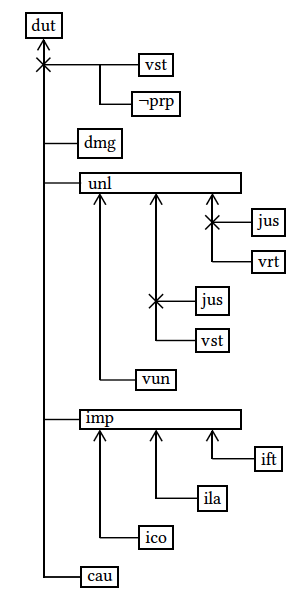
\includegraphics [scale=0.3] {figure1.png}
\caption{Arguments and their attacks in the case model of Dutch tort law}
\end{figure}

\begin{itemize}
\item $(C, \geq) \vDash dmg \wedge unl \wedge imp \wedge cau \leadsto dut \times vst \wedge \neg prp$
\item $(C, \geq) \vDash vrt \leadsto unl \times jus$
\item $(C, \geq) \vDash vst \leadsto unl \times jus$
\item $(C, \geq) \vDash vun \leadsto unl$
\item $(C, \geq) \vDash ift \leadsto imp$
\item $(C, \geq) \vDash ila \leadsto imp$
\item $(C, \geq) \vDash ico \leadsto imp$
\end{itemize}

The Dutch tort law model in the Prolog program is represented as {\mf model\_num(1)}. Through the verification given by predicate {\mf case\_model\_valid}, this model is a valid model, as shown in Figure 2. The queries about the arguments above in this model are shown in Figure 3.

\begin{figure} [htbp]
\centering
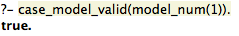
\includegraphics [scale=0.5] {model1.png}
\caption{The validity of Dutch tort law model}
\end{figure}

\begin{figure} [htbp]
\centering
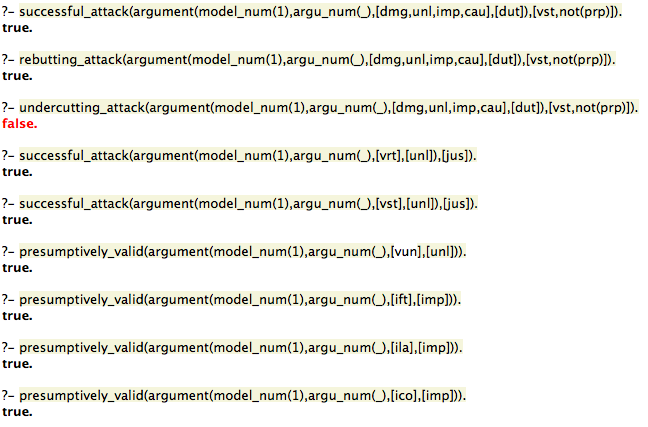
\includegraphics [scale=0.5] {ex_tort.png}
\caption{The queries in Dutch tort law model}
\end{figure}

The first query checks the validity of argument $dmg \wedge unl \wedge imp \wedge cau \leadsto dut \times vst \wedge \neg prp$ in the model. As the second and third queries shows, this attack is a rebutting attack, which means it is not undercutting. This judgement is corresponded to the analysis about the Dutch tort law model above. From the fourth query to the last one, those presumptively valid argument shown above have been verified. According to the results of the program, all of these arguments are presumptively valid.

\section{Case study: Copyright infringement in Chinese Criminal Law}

%FIRST: Explain the law informally

%SECOND: Show arguments + attacks and the associated case model

%THIRD: Show the Prolog implementation, in particular: show the validity of the arguments + attacks

\noindent The article of Copyright Infringement in Chinese Criminal Law\cite{StateCouncil2015series} is below:
\newline

\begin{adjustwidth}{0.5cm}{0cm}
\noindent \textbf{Article 217} Whoever, for the purpose of making profits, commits any of the following acts of infringement on copyright shall, if the amount of illegal gains is relatively large, or if there are other serious circumstances, be sentenced to fixed-term imprisonment of not more than three years or criminal detention and shall also, or shall only, be fined; if the amount of illegal gains is huge or if there are other especially serious circumstances, he shall be sentenced to fixed-term imprisonment of not less than three years but not more than seven years and shall also be fined:

\noindent (1) copying and publishing a written work, musical work, motion picture, television programme or other visual works, computer software or other works without permission of the copyright owner;

\noindent (2) publishing a book of which another person has the exclusive publishing right;

\noindent (3) copying and publishing audio or video recording without permission of the producer; or

\noindent (4) producing or selling an artwork where the signature of the author is forged.\newline
\end{adjustwidth}


In order to recognize the propositions in the case model easily, each elementary proposition in this model has been given an abbreviation. These abbreviations are shown in table 3.

\footnotesize
\begin{table}[htbp]
\caption{Elementary propositions in the case model of copyright infringement}
\centering
\begin{tabularx}{120mm}{>{\hsize=0.2\hsize}X>{\hsize=1.6\hsize}X}
\hline
ifg & copyright infringement\\
fpp & for the purpose of making profits\\
pac & publish and copy\\
ite & the items in Art. 217:1\\
pco & without permission of the copyright owner\\
pec & the action is not belong to "without permission of the copyright owner"\\
epr & publishing a book of which another person has the exclusive publishing right\\
avp & the audio or video recording which the producer is someone else\\
psa & producing or selling an artwork where the signature of the author is forged\\
ils & amount of illegal gains is large or other serious circumstances\\
ihe & amount of illegal gains is huge or other especially serious circumstances\\
crc & the person commits the crime of copyright infringement\\
l3fti & the person shall be sentenced to fixed-term imprisonment of not more than three years\\
cdt & the person shall be sentenced to criminal detention\\
fin & the person shall be fined\\
m3fti & the person shall be sentenced to fixed-term imprisonment of not less than three years but not more than seven years\\
hps & there is a reason which will give the defendant a heavier punishment\\
lps & there is a reason which will give the defendant a lighter punishment\\
cpb & the defendant satisfies the conditions of probation\\
pbt & the defendant will be put on probation\\
\hline
\end{tabularx}
\end{table}

\normalsize
In Art. 217, there are 4 kinds of situation in copyright infringement, if someone violates other people's copyright for the purpose of making profits, then he will be sentenced to the crime of copyright infringement. The judge will sentenced him to 4 different kinds of punishment according to the degree of severity of his crime. Above all, several rules about copyright infringement can be extracted.

If the defendant has following actions:
\begin{enumerate}
\item \textit{publish or copied something which can be considered as one of the items shown in Art. 217:1 without permission of the copyright owner};
\item \textit{publish a book of which another person has the exclusive publishing right};
\item  \textit{publish or copied the audio or video resording which the producer is someone else};
\item \textit{produce or sell an artwork where the signature of the author if forged},
\end{enumerate}
Then the defendant will be regarded as violating someone else's copyright.

If the defendant was regarded as violating someone else's copyright for the purpose of making profits, then the defendant will be sentenced to the crime of copyright infringement. This rule can be represented as $ifg \wedge fpp \Rightarrow crc$.

If \textit{the amount of defendant's illegal gains was large or existed other serious circumstances}, the defendant shall be sentenced to 3 kinds of punishments, \textit{fixed-term imprisonment of not more than 3 years and fined} ($crc \wedge ils \leadsto l3fti \wedge fin$); \textit{criminal detention and fined} ($crc \wedge ils \leadsto cdt \wedge fin$) and only \textit{fined} ($crc \wedge ils \leadsto fin$).

If \textit{the amount of defendant's illegal gains was huge or existed other especially serious circumstances}, then the defendant shall be sentenced to \textit{fixed-term imprisonment of not less that three years but not more than seven years and fined}, this can be represented as $crc \wedge ihe \Rightarrow m3fti \wedge fin$.

There are two kinds of punishments which are possible to be put on probation, if the defendant satisfied the conditions of probation: 
1. fixed-term imprisonment fo not more than 3 years and fined ($crc \wedge l3fti \wedge fin \wedge cpb \Rightarrow pbt$); 2. criminal detention and fined ($crc \wedge cdt \wedge fin \wedge cpb \Rightarrow pbt$).

According to Art. 217's relevant judicial explanations, there are 3 defeating circumstance: 1. The action is not belong to "without permission of the copyright owner"; 2. The defendant is sentenced to the crime of copyright infringement, however, he also satisfies with the conditions of being given a heavier punishment; 3. The defendant is sentenced to the crime of copyright infringement, however, he also satisfies with the conditions of being given a lighter punishment.

If we add these defeating circumstance to the rules we listed above, then some of the rules will be changed. For example,
\begin{itemize}
\item $pac \wedge ite \wedge pco \leadsto ifg \times pec$
\item $crc \wedge ils \leadsto l3fti \wedge fin \times hps$
\item $crc \wedge ihe \Rightarrow m3fti \wedge fin \times lps$
\end{itemize}

In the light of Art. 217 and the judicial explanations related to it, a case model can be built. The model has 46 cases. Case 1 is built by the principle of "presumption of innocence". Case 2 shows the scenario that although the defendant has published and copied the items shown in Art. 217:1 without the permission of the copyright owner, he still will not be considered as copyright infringement because his action is not belong to "without permission of the copyright owner". Case 3 shows the scenario that the defendant violated someone else's copyright, but he didn't do it for making profits, so he will not be judge through Art. 217.

From Case 4 to Case 13, different punishments for the defendant's action in Art. 217:1 are listed. In the same way, different punishments for the defendant in Art. 217:2, Art. 217:3 and Art. 217:4 will also be listed into the case model. Table 4 lists cases from Case 1 to Case 13. Case 14 to Case 46 have similar components with Case 4 to Case 13, except the acts of infringement on copyright are different.

\footnotesize
\begin{table}[htb]
\caption{The case list of the case model}
\centering
\begin{tabularx}{120mm}{>{\hsize=0.1\hsize}X>{\hsize=1.6\hsize}X}
\hline
1	& $\neg$pac, $\neg$ite, $\neg$pco, $\neg$epr, $\neg$avp, $\neg$psa, $\neg$ifg \\
2	& pac, ite, pco, pec, $\neg$ifg \\
3	& pac, ite, pco, $\neg$pec, $\neg$epr, $\neg$avp, $\neg$psa, ifg, $\neg$fpp \\
4	& pac, ite, pco, $\neg$epr, $\neg$avp, $\neg$psa, ifg, fpp, ihe, $\neg$ils, crc, hps, $\neg$lps, $\neg$m3fti, $\neg$l3fti, $\neg$cdt, $\neg$fin \\
5	& pac, ite, pco, $\neg$epr, $\neg$avp, $\neg$psa, ifg, fpp, ihe, $\neg$ils, crc, $\neg$hps, lps, $\neg$m3fti, $\neg$l3fti, $\neg$cdt, $\neg$fin \\
6	& pac, ite, pco, $\neg$epr, $\neg$avp, $\neg$psa, ifg, fpp, ihe, $\neg$ils, crc, $\neg$hps, $\neg$lps, m3fti, $\neg$l3fti, $\neg$cdt, fin \\
7	& pac, ite, pco, $\neg$epr, $\neg$avp, $\neg$psa, ifg, fpp, $\neg$ihe, ils, crc, hps, $\neg$lps, $\neg$m3fti, $\neg$l3fti, $\neg$cdt, $\neg$fin \\
8	& pac, ite, pco, $\neg$epr, $\neg$avp, $\neg$psa, ifg, fpp, $\neg$ihe, ils, crc, $\neg$hps, lps, $\neg$m3fti, $\neg$l3fti, $\neg$cdt, $\neg$fin \\
9	& pac, ite, pco, $\neg$epr, $\neg$avp, $\neg$psa, ifg, fpp, $\neg$ihe, ils, crc, $\neg$hps, $\neg$lps, $\neg$m3fti, $\neg$l3fti, $\neg$cdt, fin \\
10	& pac, ite, pco, $\neg$epr, $\neg$avp, $\neg$psa, ifg, fpp, $\neg$ihe, ils, crc, $\neg$hps, $\neg$lps, $\neg$m3fti, l3fti, $\neg$cdt, fin, cpb, pbt \\
11	& pac, ite, pco, $\neg$epr, $\neg$avp, $\neg$psa, ifg, fpp, $\neg$ihe, ils, crc, $\neg$hps, $\neg$lps, $\neg$m3fti, $\neg$l3fti, cdt, fin, cpb, pbt \\
12	& pac, ite, pco, $\neg$epr, $\neg$avp, $\neg$psa, ifg, fpp, $\neg$ihe, ils, crc, $\neg$hps, $\neg$lps, $\neg$m3fti, l3fti, $\neg$cdt, fin, $\neg$cpb, $\neg$pbt \\
13	& pac, ite, pco, $\neg$epr, $\neg$avp, $\neg$psa, ifg, fpp, $\neg$ihe, ils, crc, $\neg$hps, $\neg$lps, $\neg$m3fti, $\neg$l3fti, cdt, fin, $\neg$cpb, $\neg$pbt \\
14	& ... ... \\ 
\hline
Order & case 1 $>$ case 2 = case 3 = case 14 = case 25 = case 36 $>$ case 4 = case 5 = case 7 = case 8 = case 15 = case 16 = case 18 = case 19 = case 26 = case 27 = case 29 = case 30 = case 37 = case 38 = case 40 = case 41 $>$ case 6 = case 9 = case 10 = case 11 = case 12 = case 13 = case 17 = case 20 = case 21 = case 22 = case 23 = case 24 = case 28 = case 31 = case 32 = case 33 = case 34 = case 35 = case 39 = case 42 = case 43 = case 44 = case 45 = case 46\\
\hline
\end{tabularx}
\end{table}

\normalsize
From this copyright infringement model, we can get the argument diagram illustrated in Figure 4. This argument has multi-steps, and it is corresponding to the model we built.

\begin{figure} [htbp]
\centering
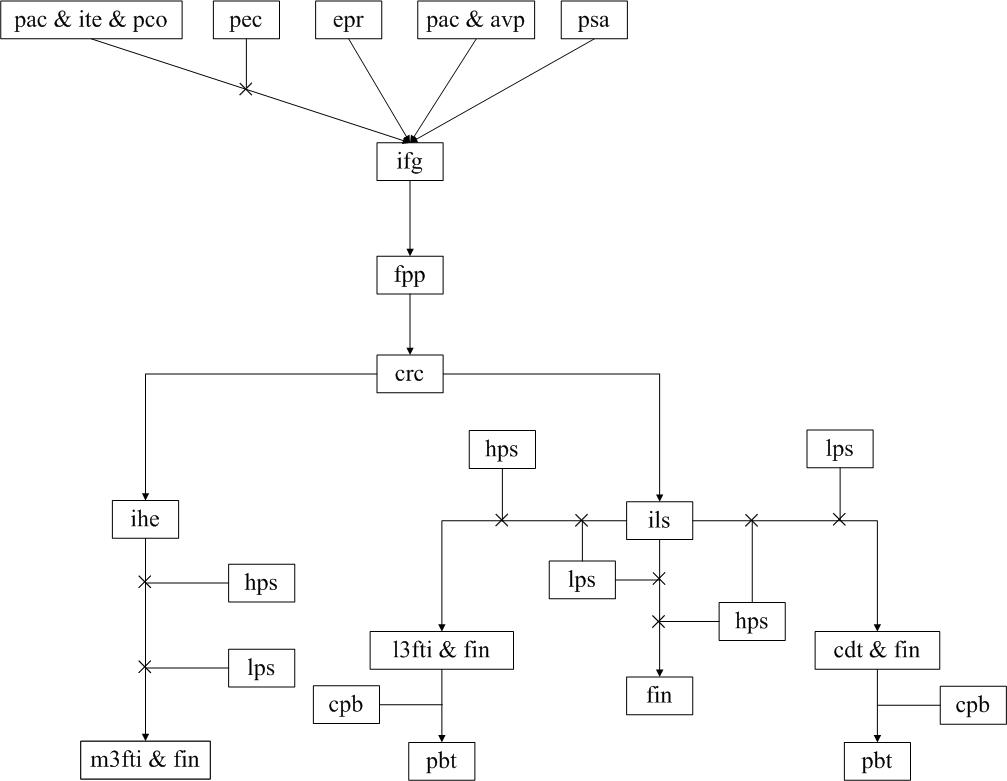
\includegraphics [scale=0.32] {argument_diagram1.jpg}
\caption{Arguments and their attacks in the case model of Chinese copyright infringement}
\end{figure}

According to the definitions of Verheij's case model formalism, the rule $epr \Rightarrow ifg$ is valid in this model. As the model shows, case 14 and case 15 implicate sentence $epr \wedge ifg$ which is the case made by the argument $(epr, ifg)$, so this argument is coherent. Besides, all the cases which imply the premise $epr$, also imply the conclusion $ifg$. So argument $(epr, ifg)$ is conclusive in the case model. And these arguments are also conclusive in the model:

\begin{itemize}
\item $(C,  \geq) \models pac \wedge avp \Rightarrow ifg$
\item $(C,  \geq) \models ifg \wedge fpp \Rightarrow crc$
\item $(C,  \geq) \models crc \wedge l3fti \wedge fin \wedge cpb \Rightarrow pbt$
\end{itemize}

According to the definitions of Verheij's case model formalism, the rule $pac \wedge ite \wedge pco \leadsto ifg \times pec$ is also valid in the copyright infringement model. The attack from $pec$ successfully attacked the presumptively valid argument $(pac \wedge ite \wedge pco, ifg)$, and made the argument $(pac \wedge ite \wedge pco \wedge pec, \neg ifg)$ presumptively valid. In the light of the copyright infringement model, Case 2 has implied the case made by the argument $(pac \wedge ite \wedge pco \wedge pec, \neg ifg)$, so this argument is coherent. Furthermore, Case 2 is the strongest case in the cases which implied the premise of this argument. So we say the argument $(pac \wedge ite \wedge pco \wedge pec, \neg ifg)$ is presumptively valid in the case model. The arguments below are also presumptively valid:

\begin{itemize}
\item $(C,  \subseteq) \models crc \wedge ils \leadsto l3fti \wedge fin \times hps$
\item $(C,  \subseteq) \models crc \wedge ils \leadsto cdt \wedge fin \times hps$
\item $(C,  \subseteq) \models crc \wedge ihe \leadsto m3fti \wedge fin \times lps$
\end{itemize}

The Chinese copyright infringement model is represented as {\mf model\_num(2)} in the program. Figure 5 shows that it is a valid model. The arguments and attacks shown above can be verified by this program.

\begin{figure} [htbp]
\centering
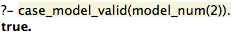
\includegraphics [scale=0.5] {model2.png}
\caption{The validity of Chinese copyright infringement model}
\end{figure}

\begin{figure} [htbp]
\centering
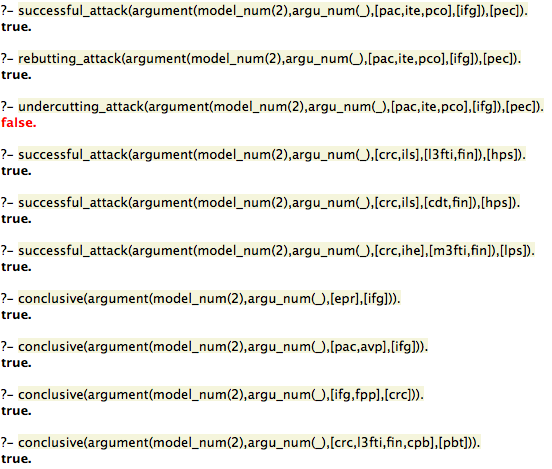
\includegraphics [scale=0.5] {ex_copyright.png}
\caption{The queries in Chinese copyright infringement model}
\end{figure}

As Figure 6 shows, the program has verified that circumstance \textit{pec} successfully attack argument $pac \wedge ite \wedge pco \leadsto ifg$, and it is a rebutting attack, as well as the other arguments with defeating circumstances above which are also considered to be successful. The program also finds argument $epr \Rightarrow ifg$ and other three arguments to be conclusive. These results are corresponded to the analysis about Chinese copyright infringement model above.

\section{Discussion and Conclusion}

\noindent In this paper, two case models with different backgrounds based on Verheij's case model formalism have been discussed. As the arguments implied in these case models are corresponded to the rules in statutes, Verheij's theory has been proved that it is suitable for Chinese legal system. The preferred relation established by Verheij solves the priority relationship among the cases in case model, so that the presumptive arguments in legal reasoning can be concluded by this theory. In other words, some legal issues can be solved, such as the rules used for legal reasoning, which are beyond the statutes, for instance, "presumption of innocence" in the background of Chinese legal system. Although it is not in any statute, every judge will think about it during the process of making decisions. So we can place this rule as several cases in the preferred relation of a case model properly to solve this issue. Therefore, we believe arguments embedded values are more suitable for dealing with practical issues in legal reasoning. 

The program we build in this paper intends to make the modeling process with less mistakes and its main function is automatically verifying the validity of the arguments implicated in a case model and the case model itself. This program has been proved that it is completely suitable for those models based on Verheij's theory, even these models have different backgrounds. Compare with the original hand-made modeling way, it can reduce mistakes during the process of modeling significantly, as this program can verify the model automatically. So, it is a successful attempt as a computational implementation for Verheij's case model formalism which can make Verheij's theory more useable in practical environment. 

However, there is still room for improvement. For those people who are unfamiliar with legal statues, an explicit case model can be helpful for them, which means the model needs to contain as much details as possible, such as the official judicial explanations related to Chinese criminal law. But this action can bring a problem cannot be ignored. For instance, there are 8 scenarios about the elementary proposition "amount of illegal gains is huge or other especially serious circumstances" mentioned in the Chinese copyright infringement model in the light of relevant judicial explanations, if all of these specific scenarios are added into the model, the number of cases in this model will become huge. According to the way of building a model completely based on Verheij's formalism, all these scenarios will be treated as elementary propositions and they will replace the position of  $ihe$. The number of cases will increase by eight times, if we added these specific scenarios to the model by Verheij's theory directly, which also lets the process of modeling easily to make mistakes. It will be a hard job for the people who wants to build a model. This issue needed to be solved in the future research.

The results of this paper shows that Verheij's case model formalism can be used to model the object with complex argument structure, and the program developed in this paper is feasible for the models based on Verheij's theory. It also proves that the Prolog program we built can well combine cases, rules and arguments. It is not only applicable to the civil law system but also to the Chinese legal system. AI and legal reasoning technology needs to combine rule-based reasoning, case-based reasoning and argumentation together, and argumentation technology can be the bridge of both cases and rules.

\footnotesize
\bibliographystyle{unsrt}
\setcitestyle{round,aysep={},yysep={;}}
\bibliography{AIandLaw}
\normalsize
\end{document}